%%% Local Variables: 
%%% coding: utf-8
%%% mode: latex
%%% TeX-engine: xetex
%%% End:

% main.tex файл который компилируется и подключает за собой остальный
% файлы с содержимым через input
% При этом согласно моей же логике преамбула должна отстаться здесь.

% Используем опцию emptystyle т.к. bsuir-std расширяет eskdxtext,
% который без этой опции сделает рамку для чертежа даже на документе
% с просто текстом.
\documentclass[a4paper,emptystyle]{bsuir-std}


% BibLaTeX нужен для библиографии
\usepackage[backend=biber,sorting=none]{biblatex}
% Эта штука рекомендуется вместе с biblatex
\usepackage{csquotes}


% Добавляем файл с библиографией
\addbibresource{Karakin5semCoursework.bib}


\begin{document}

% Путь к месту где картинки лежат
\graphicspath{ {images/} }

%%% Титульник
%%% Local Variables: 
%%% coding: utf-8
%%% mode: latex
%%% TeX-engine: xetex
%%% End:

%%% Титульный лист

\begin{titlepage}
  % Устаналиваем стиль ESKD empty, иначе на титульнике будет стоять
  % номер страницы. Потому что в классе bsuir-std я включил нумерацию.
  \ESKDstyle{empty}
  \ESKDthisStyle{empty}
\begin{center}
Министерство образования Республики Беларусь\\[1.2em]
Учреждение образования\\[0.4em]
БЕЛОРУССКИЙ ГОСУДАРСТВЕННЫЙ УНИВЕРСИТЕТ ИНФОРМАТИКИ И РАДИОЭЛЕКТРОНИКИ\\[2.0em]
\end{center}
Факультет компьютерного проектирования\\
Кафедра проектирования информационно-компьютерных систем

\begin{flushright}
  \begin{minipage}{0.5\textwidth}
    \textit{К защите допустить:}\\
    Руководитель курсового проекта\\
    Доцент, к.т.н.\\
    \underline{\hspace*{2.8cm}} Г.\,А.~Пискун
  \end{minipage}\\[2em]
\end{flushright}

\begin{center}
  \textbf{ПОЯСНИТЕЛЬНАЯ ЗАПИСКА}\\
  к курсовому проекту\\
  на тему\\[2.0em]

  \textbf{БЕСПРОВОДНОЙ РОУТЕР АССИМЕТРИЧНОЙ ЦИФРОВОЙ АБОНЕНТСКОЙ ЛИНИИ}\\
\end{center}
\end{titlepage}



%%% Введение.
\begin{center}
\textbf{ВВЕДЕНИЕ}
\end{center}

\par
Беспроводной роутер ассиметричной цифровой абонентской линии — это
устройство предназначенное для предоставления доступа в интернет.
\par
Пользовательские устройства подключаются к роутеру по протоколу
беспроводной связи, а сам роутер включается в сеть интернет-провайдера
по модемной технологии ассиметричной цифровой абонентской линии.
Ассиметричность цифровой абонентской линии означает то, что исходящая
пропускная полоса канала связи может быть не равна входящей.
\par
В данном случае роутер предоставляет доступ в интернет в пределах
одного дома, квартиры или небольшого офиса.
Однако даже для того, чтобы обеспечить работу даже в пределах
небольшой домашней сети, требуются вычислительные ресурсы,
которые используются роутером для выполнения задач
по обеспечению работоспособности сети.
\par
В такие типовые задачи роутера входит:
\begin{itemize}[nosep]

\item Трансляция сетевых адресов;
\item Динамическая конфигурация подключаемых устройств;
\item Фильтрация сетевых пакетов.
\end{itemize}
\par
В результате работы роутер нагревается, а охлаждение этого устройства
является основной темой данной курсовой работы.
\par
Цель данной курсовой работы — обосновать эффективность выбранной
системы охлаждения, для беспроводного роутера ассиметричной цифровой
абонентской линии 68.4 мВт, 12 В, модель ASW800 ADSL.
Задача курсовой работы – провести анализ теплового режима
радиоэлектронного средства в негерметичном перфарированным корпусом,
охлаждаемого с помощью естественной вентиляцией, и на основании
полученных результатов расчетов сделать вывод об эффективности
выбранного метода охлаждения.
\par
В курсовой работе использовались такие методы исследования, как:
\begin{itemize}[nosep]
\item аналитический;
\item физико-математический;
\item метод моделирования и компьютерной обработки данных.  
\end{itemize}

\par
В первом разделе курсовой работы рассматривается и анализируется
устройство и его внутренние компоненты, по которым производится
расчёт теплового режима. Во втором разделе производятся расчеты
теплового режима РЭС и краткий анализ полученных данных.
В третьем разделе описывается процесс модерилования тепловой
картины поля микросхемы РЭС, описывается программный комплекс для моделирования.
В четвертом разделе сравниваются и анализируются данные, полученные при расчете
и определяется адекватность полученных данных.

\newpage

%%% Первая глава
\section{ОБЩЕТЕХНИЧЕСКИЙ АНАЛИЗ ПРОЕКТИРУЕМОГО УСТРОЙСТВА}
\subsection{Анализ исходных данных}
\par
В курсовой работе рассматривается беспроводной роутер асимметричной
цифровой абонентской линии.  Чтобы кратко сформулировать назначение
данного сетевого устройства достаточно одного слова — маршрутизатор.
Потому что именно задачу маршрутизации, то есть доставки сетевых
пакетов из пользовательской сети в сеть интернет-провайдера решают
такого рода устройства.
\par
Одной из функций маршрутизатора является физическогое соединение
сетей. Маршрутизатор имеет несколько сетевых интерфейсов, подобных
интерфейсам компьютера, к каждому из которых может быть подключена
одна сеть. Маршрутизатор может быть реализован программно на базе
универсального компьютера (например, типовая конфигурация Unix или
Windows включает программный модуль маршрутизатора). Однако чаще
маршрутизаторы реализуются на базе специализированных аппаратных
платформ. В состав программного обеспечения маршрутизатора входят
протокольные модули сетевого уровня ~\cite{NetworksOlifer2016}.

Роутер выполнен в виде платы с распаянными компонентами, в
негерметичном корпусе с перфорацией для обеспечения естественной
вентиляции РЭС. Корпус имеет форму параллелепипида, на задней панели
содержит разъём RJ-45 для подключения к телефонной сети и четыре
разъёма для подключения по стандарту Ethernet, антенну, разъём питания
и тумблер включения.

\begin{figure}[h] %% h means here
  \centering
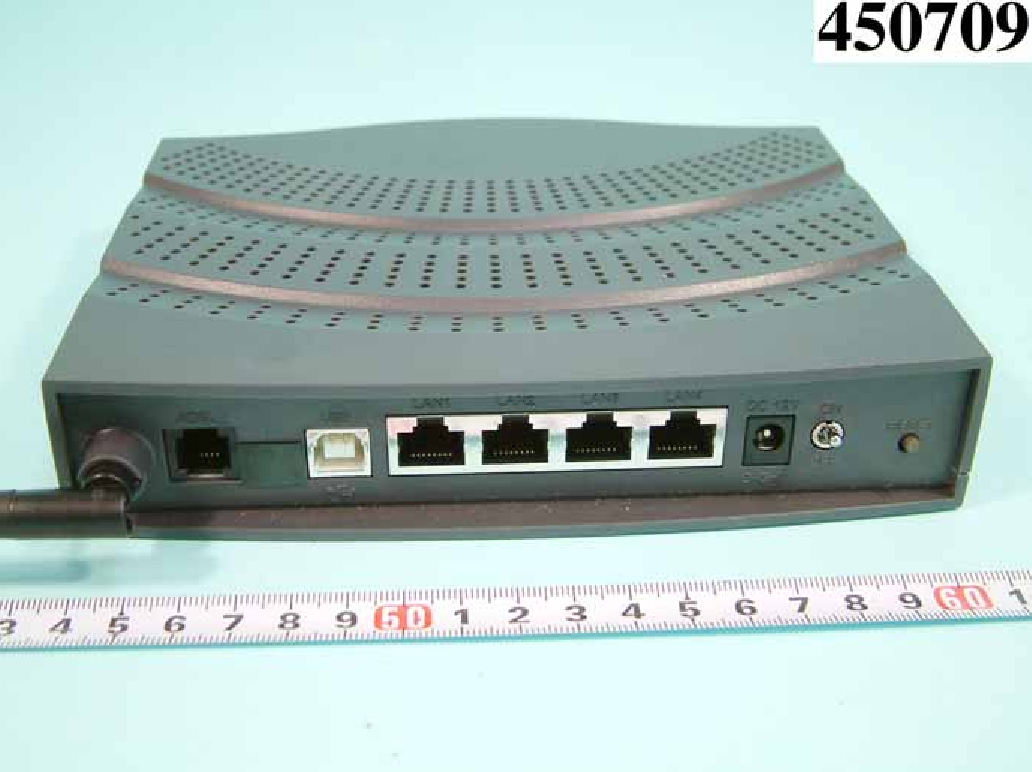
\includegraphics[scale = 0.7]{external_photos-2.png}
\caption{Фотография задней панели роутера ~\cite{EXTERNAL_PHOTOS}.}

\end{figure}

Поскольку в курсовой работе будет производиться расчёт тепловых
режимов будет также важно учитывать климатические факторы внешней
среды, то какие условия эксплутации при этом должны быть соблюдены
регламентирует соответсвующий стандарт — ГОСТ 15150-69
~\cite{GOST_15150-69}.

Настоящий стандарт должен применяться при проектировании изделий.  В
частности, он должен применяться при состалвении технических заданий
на разработку или модернизацию изделий, а также при разработке
государственных стандартов и технических условий, устанавливающих
требования в части воздействия климатических факторов внешней среды
для группы изделий, а при отсуствии указанных групповых документов —
для отдельных видов изделий ~\cite{GOST_15150-69}.

Для конкретных типов или групп изделий виды воздействующих
климатических факторов и их номинальные значения устанавливаются в
зависимости от условий эксплуатации изделий в соответвующих
технических заданих, стандартах и технических условиях ~\cite{GOST_15150-69}.

Так как в данном случае роутер предоставляет доступ в интернет в
пределах одного дома, квартиры или небольшого офиса. Можно говорить, что роутер соответствует категории УХЛ4.2 ГОСТ15150-69.

Характеристика данной категории следующая:\\
Для эксплуатации в помещниях (объемах) с искуственно регулируемыми
климатическими условиями, например в закрытых отапливаемых или
охлаждаемых и вентелируемых производственных и других, в том числе
хорошо вентилиуруемых подземных помещниях (отсуствие воздействия
прямого соленчного излучения, атмосферных осадков, ветра, песка и пыли
наружного воздуха; отсутвие или существенное уменьшение воздействия
рассеяного солнечного излучения и конденсации влаги). Для эксплуатации
в лабораторных, капитальных и других подобного типа помещениях ~\cite{GOST_15150-69}.

Соответствие условий работы роутера ассиметричной цифровой абонетской
линии данному ГОСТ важно по той причине, что климатические условия
регламентиуремые ГОСТ влияют на внешние тепловые воздействия на РЭС.
В зависимости от них также может быть выбран корпус определённого
типа.

\subsection{Описание принципа работы анализируемого устройства}


Рассмотренной устройство — специализированная аппартная платформа,
реализующего фукнции маршрутизатора в сетевой топологии.  Чтобы ещё
больше конкретизировать назначение устройства необходимо упомянуть в
каком сегменте сети оно осуществляет свою работу.


Локальная сеть (LAN, Local Area Network) — частная сеть,
функционирующая в отдельном здании и на прилегающей территории
(это может быть дом, офис или завод). LAN широко применяется для соединения персоналтьны компьютеров и бытовой электроники, позволяя совместно
использовать различные ресурсы (например, принтеры) и обмениваться
информацией ~\cite{NetworksTanenbaum2023}.

На сегодняшний день беспроводные LAN применяются
повсеместно. Изначально они были популярны в жилых помещениях, старых
офисных зданиях, кафе и других местах, где прокладка кабелей обошлась
бы слишком дорого. В подобных система компьютеры обмениваются
информацией с помощью встроенного радиомодема и антенны. Чаще всего
компьютер обращается к специальному устройству, которой называется
точкой доступа (AP, Access Point), беспроводным маршрутизатором
(wireless router) или базовой станцией (base station). Это устройство
осуществляет передачу пакетов данных между беспроводными компьютерами,
а также между компьютером и интернетом. Точка доступа напоминает
популярного ребенка в школе, поскольку все хотят с ней «поговорить»
~\cite{NetworksTanenbaum2023}.

Одним из самых популярных стандартов беспроводных LAN является IEEE
802.11, более известный как wi-fi ~\cite{NetworksTanenbaum2023}.

И именно этому стандарту следует рассматриваемое устройство.

Вместо дорогостоящих лицензируемых частот системы 802.11 работают на
нелицензируемых полосах частот, например ISM («Industrial, Scientific,
and Medical» — «промышленные, научные и медицинские») устанавливаемых
МСЭ-R (например 902-928 МГц, 2,4-2,5 ГГц, 5,725-5,825 ГГц).  Этот
диапазон частот разрешено использовать любым устройствам, но мощность
их излучения должна быть ограничена, чтобы различные устройства не
мешали друг другу. Конечно, из-за этого 802.11-передатчики иногда
начинают конкурировать за частоты с беспроводными телефонами,
системами дистанционного открывания дверей гаража и микроволновками.
Так что до тех пор, пока пользователям не понадобиться позвонить
гаражным дверям, важно все настроить
правильно ~\cite{NetworksTanenbaum2023}.

Таким образом рассмотренное устройства это РЭС основная задача
которого — это прием, модуляция, обработка и передача сигнала другим
устройствам и аппаратуре. При этом, поскольку устройство производит не
только физическую передачу данных, но и коммутацию сетевых пакетов,
оказываются нужными некоторые вычислительные ресурсы.
Следовательно для того чтобы осуществлять вычисления устройство будет
оснащенно микропроцессором.

\subsection{Анализ элементной базы устройства}

Используя блок схему рассмотрим элементную базу
маршрутизатора.


\begin{figure}[h] %% h means here
  \centering
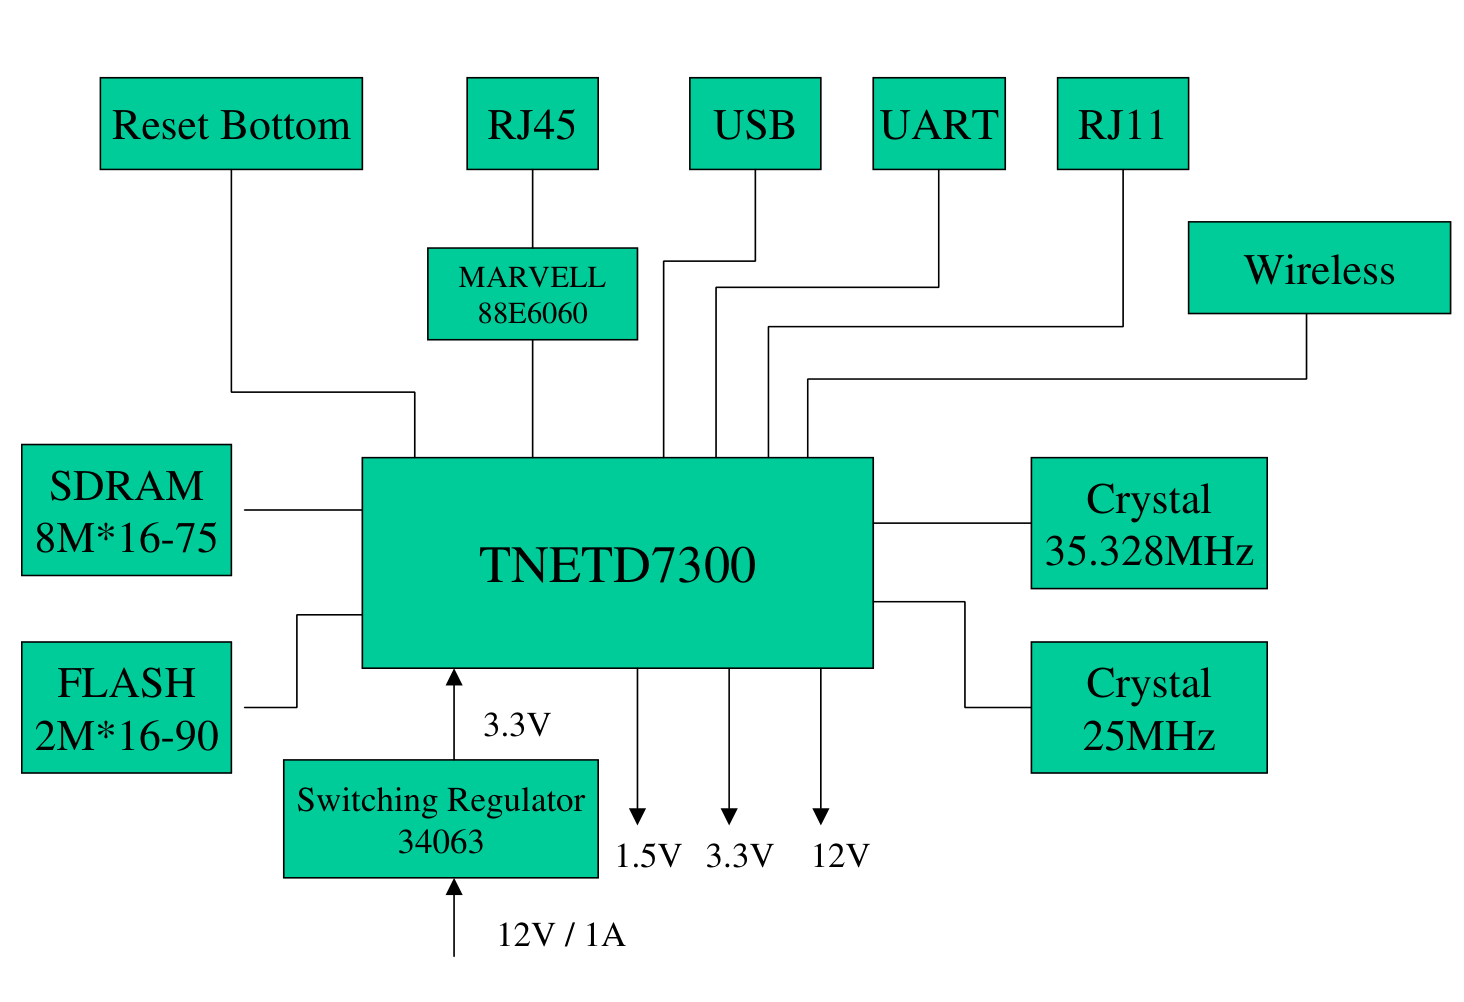
\includegraphics[scale = 0.7]{block_diagram-0.png}
\caption{Блок схема устройства маршрутизатора ASW800ADSL ~\cite{BLOCK_DIAGRAM}.}
\end{figure}
 
Как видно из блок схемы первостепенным и самым важным модулем данной
РЭС явяляется чип TNETD7300, он расположен в цетрне блок схемы. С ним
соеденены несколько интерфейсов и остальные модули.

Из того как расположен этот модуль на блоксхеме можно сделать вывод,
что в этой части РЭС будет рассеиваться больше всего мощности.

Различают внтуренние и внешние тепловые воздействия на РЭА.
Внутренние тепловые воздействия на РЭА в основном зависят от мощности
рассеиваемой её элементами ~\cite{Rotkop1976}.

Энергетический коэффициент полезного действия радиоэлементов, как
правило, невелик, и значительная доля энергии питания превращается в
тепловую энергию с сопутствующим перегревом элементов и аппаратуры
~\cite{Rotkop1976}.

Насыщение современных технических устройств РЭА различного назначения
заставляет конструкторов уменьшать ее габариты и увеличивать удельные
мощности рассеивания, т.е. мощности, приходящиеся на единицу
поверхности или объема РЭА. Одним из основных направлений в
конструировании РЭА стала комплексная микроминиатюризация, что
приводит к ещё большему увелечению удельной мощности рассеивания
~\cite{Rotkop1976}.

%% \pagebreak
Рассмотрим схему электрическую принципиальную на которой изображён чип
TNETD7300.

\begin{figure}[hb]
  \centering
  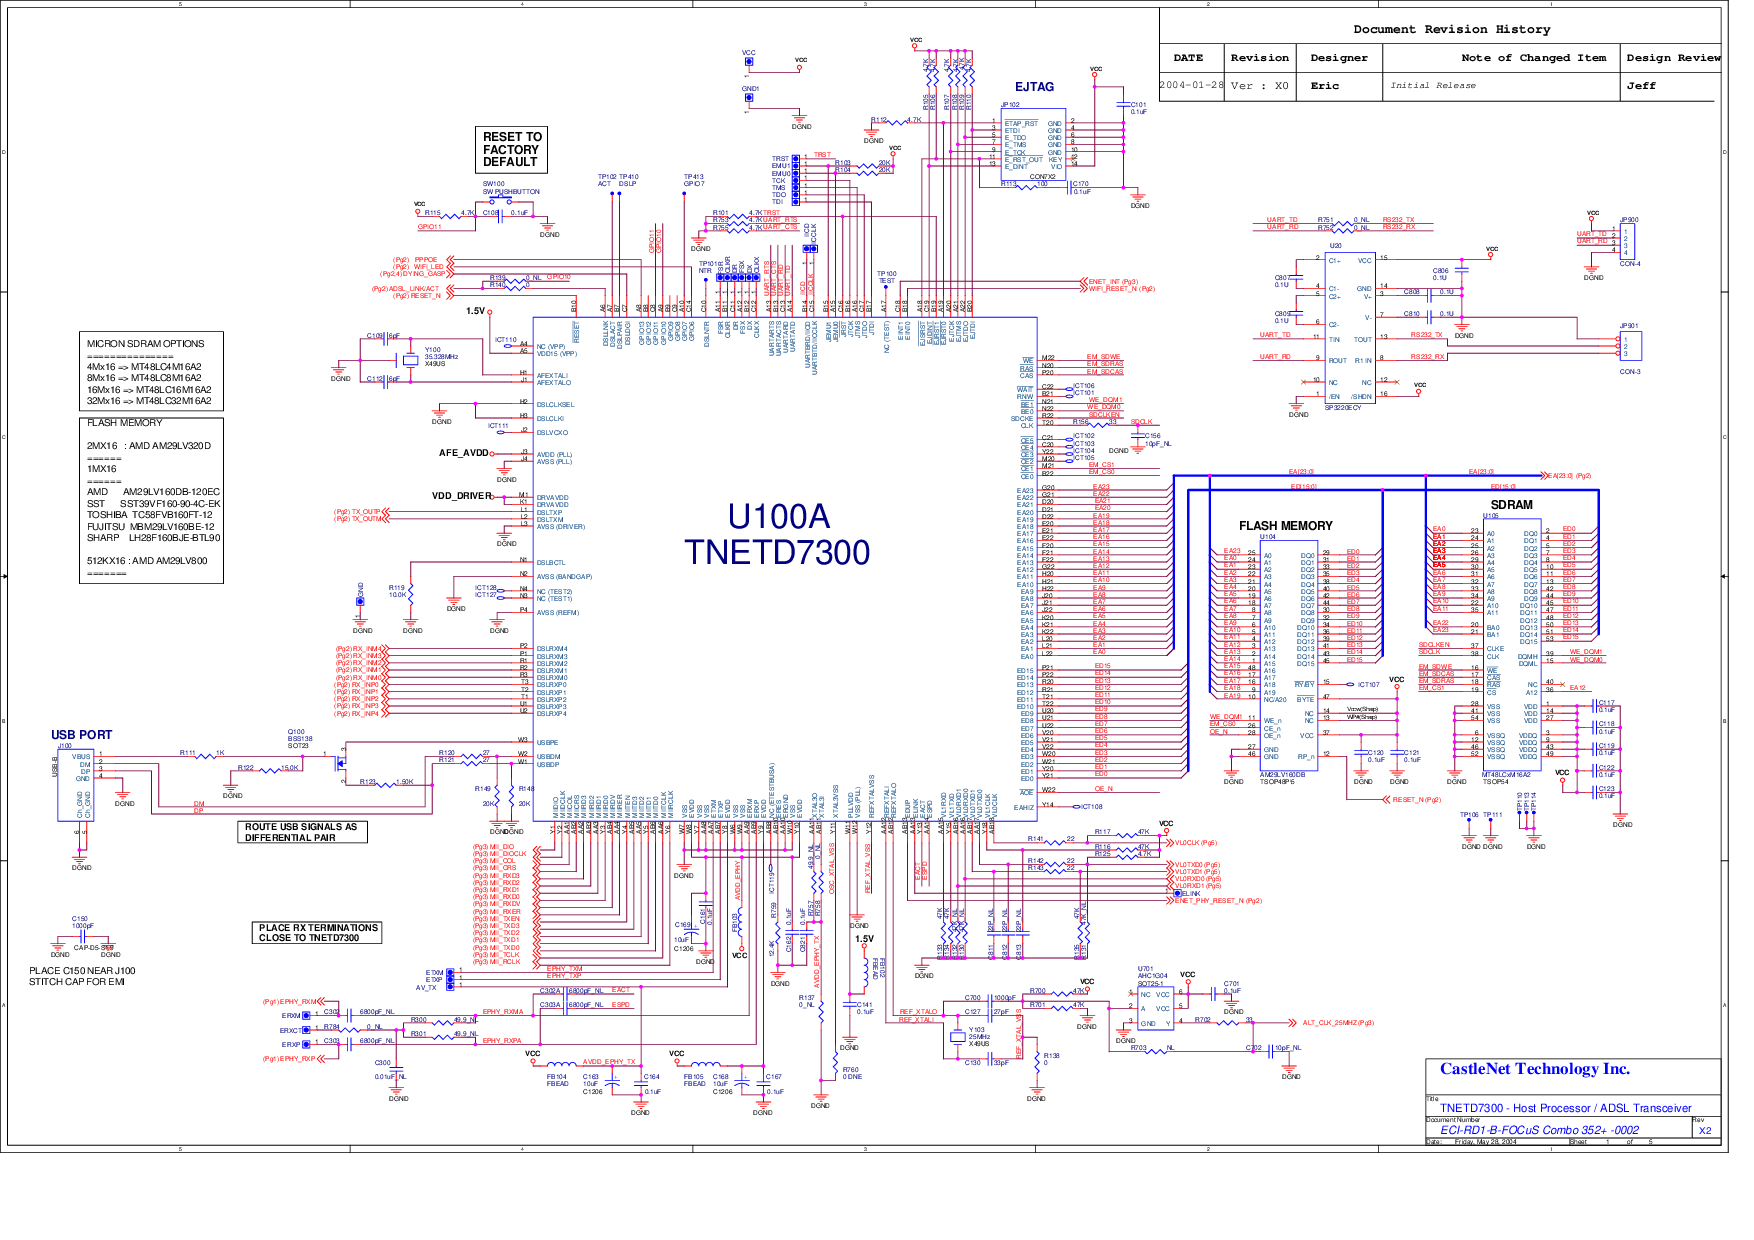
\includegraphics[scale = 0.25]{schematics-1.png}
  \caption{Схема электрическая принципиальная
    маршрутизатора ASW800ADSL ~\cite{SCHEMATICS}.}
\end{figure}

На схеме чип TNETD7300 подписан не иначе как \textit{«Host Proccessor»}.
Из этого можно сделать вывод, что, уже упомянутым в предыдущем
параграфе, микропроцессором и будет являться этот чип.  На схеме
электрической принципиальной микропроцессор выглядит как квадрат к
которому подведены другие компоненты. Такой способ изображения вызван
тем, что для того чтобы показать все элементы из которых состоит
процессор требуется отдельная большая подсхема, которая в свою очередь
была бы разделена на несколько других подсхем соответствующих
отдельным частями процессора, таким как арифметико логическое
устройство, блок управления памятью и другие. Это ещё раз подтверждает
вывод о том, что данное устройство рассеивает больше всего мощности, а
значит и требует наибольшего охлаждения.

\subsection{Выбор и обоснование системы охлаждения}

Защита от тепловых воздействий это одна из важных задач решаемых в обеспечении недёжности РЭС.

Защита РЭА от тепловых воздействий осуществляется при помощи ряда мероприйтий. Одним из основных является использование систем обеспечения теплового режима РЭА (СОТР). СОТР обычно предназначена для поддержания заданного в технических условиях (ТУ) диапазона температур на элементах РЭА, чтобы обеспечить ее надежность при определенных тепловых воздействиях и других специальных требованиях ~\cite{Rotkop1976}.

В радиоэлектронных комплексах СОТР, как правило, являются сложными
системами, состоящими из многих элементов, коммуникациий и несущих
конструкий. В некоторых случаях регулирование температуры в РЭА может
быть достигнуто за счет простейших конструктивных решений,
осущствляющих теплопередачу между элементами РЭА, элементами несущей
конструкции и окружающей средой. Тогда нет смысла рассматривать СОТР
как отдельное изделие и мы будем пользоваться терминами «методы (или
спосбы) охлаждения РЭА». Этими же терминами будем пользоваться и при
исследовании температурного поля элементов РЭА, в результате действия
некоторых гипотетических СОТР, когда конкретная конструкция СОТР не
рассматривается ~\cite{Rotkop1976}.

Для выбора и обоснование системы охлаждения важно иметь представление
о тепловом режиме РЭС.
Тепловой режим есть совокупность значений температур в различных
точках всей РЭС, её корпуса и СОТР.



\section{Расчет теплового режима РЭС при естественном воздушном охлаждении.}
%% 4.2

Расчет теполового режима радиоэлектронных аппартов рекомендуется
проводить в три этапа~\cite{Rotkop1976}:
\begin{enumerate}[label={\arabic*.}]
  \item Определение среднеповерхностной температуры платы с
расположенными ней деталями, корпуса и температуры воздуха внтури
радиоэлектронного аппарата.
  \item Определить среднеповерхностные температуры корпусов элементов
  используя результаты первого этапа.
  \item Определить максимальные температуры критических зон элементов и
их функциональные связи со среднеповерхностной температурой как
корпусов, так и и плат.
\end{enumerate}

Первый и второй этапы расчета позволяют получить значения основных
параметров, связанных с выбором системы охлаждения, т.е. первых двух
этапов хватает для принятия конструкторсого решения касаемо выбора
системы охлаждения.

Полную систему уравнений теплообмена для реального аппарата часто
невозможно не только решить аналитически, но и строго записать. В
связи с этим процессы, протекающие в реальном радиоэлектронном
аппарате, схематизируют, принимают ряд упрощающик предпосылок и в
результате получают тепловую модель аппарата, для которой и проводят
рассчет теплового режима ~\cite{Rotkop1976}.

Наибольшее распространение получила весьма плодотворная схематичзация
процессов теплообмена в РЭА, предложенная Г.Н.Дульневым
~\cite{Dulnev1968}.

Суть метода заключается в том, что печатная плата с её элементами
принимается за одно тело с изотермической поверхностью (нагретую
зону), для которого и проводится расчет теплового режима.

Таким образом производится расчет среднеповерхностной температуры
нагретой зоны.

Под понятием нагретая зона понимается поверхность того элемента на
печатной плате, который рассеивает больше всего мощности.

В данном случае им является процессор ТNETD 7300.

В указанных ранее источниках нет инфомации о том каковы размеры это
чипа. Однако согласно буклету производителя данный чип принадлежит к
вычислительной архитектуре RISC MIPS 32 ~\cite{AR7_fact_sheet}.

Понимание того, к какой архитектуре относится процессор позволяет
определить чипсет, который им используется. В свою очередь данные о
чипсете позволяют сделать вывод о том какова площадь процессора.

Чипсет, размещаемый на материнской плате, выполняет функцию связующего
компонента (моста), обеспечивающего взаимодействие центрального
процессора (ЦП) c различными типами памяти, устройствами ввода-вывода,
контроллерами, как непосредственно через себя, так и через другие
контроллеры и адаптеры, с помощью многоуровневой системы
шин~\cite{Avdeev2019}.

Без чипсета процессор не сможет взаимодествовать с переферийными
устройствами напрямую.

Исходя из даты изготовления всей РЭС и архитекутры конкретного чипа,
можно сделать вывод, что процессор размещается на чипсете R8000
~\cite{R8000_physical_wikipedia}.

Согласно этим данным чипсет имеет форму прямоугольника со сторонами в
$l_1$ = 17,34 мм и $l_2$ = 17,30 мм (занимает площадь 299,98 мм$^2$) и
рассеивает 13 ват мощности.

Основываясь на информации о процессорах тех лет, примем высоту чипа
$l_3$ равной 2,5 мм ~\cite{MobilePentium3_wikipedia}.

Таким образом можно найти условную поверхность нагретой зоны по
формуле:

\begin{equation}
S \mathrm{_з} = 2 (l_1 l_2 + (l_1 + l_2) l_3 K \mathrm{_з} )
\end{equation}

\subsection{Расчет теплового режима РЭС в герметичном корпусе}
%% 4.2.1

\subsection{Расчет теплового режима РЭС в герметичном корпусе с внутренним перемешиванием}
%% 4.2.2.

\subsection{Расчет теплового режима РЭС в герметичном корпусе с наружным обдувом}
%% 4.2.3.

\subsection{Расчет теплового режима РЭС в герметичном оребрённом корпусе}
%% 4.2.4

\subsection{Расчет теплового режима РЭС в перфорированном корпусе}
%% 4.2.5

\subsection{Расчет теплового режима РЭС при принудительном охлаждении}%% 4.2.6

\end{document}
